% !Mode:: "TeX:UTF-8"
% !TEX program  = xelatex

%\documentclass{cumcmthesis}
\documentclass[withoutpreface,bwprint]{cumcmthesis}%去掉封面与编号页,电子版提交的时候使用。


\usepackage{algorithm}
\usepackage{algorithmic}
\usepackage[framemethod=TikZ]{mdframed}
\usepackage{url}   % 网页链接
\usepackage{subcaption} % 子标题
\title{古代玻璃制品的成分分析与鉴别}
\tihao{C}
\baominghao{202219025023}
\schoolname{广东第二师范学院}
\membera{余树洪}
\memberb{邓明蔚}
\memberc{黄惠娟}
\supervisor{廖建全}
\yearinput{2022}
\monthinput{09}
\dayinput{18}

\begin{document}
	
	\maketitle
	
	\begin{abstract}
		本文针对古代文物玻璃饰品的化学成分分析进行分析以及玻璃饰品的类型鉴别,根据已有的数据基础下,根据表单1的数据,建立表层风化-相关特征评估模型,分析表层风化与其玻璃类型、纹饰和颜色之间的关系,利用卡方检验和相关性分析综合评价表层风化与其他三个特征变量的关系。然后根据附件的数据的文物化学成分数据来建立相关的模型算法,探索古代文物玻璃饰品的玻璃类型与其化学成分的关系。
		
		在建立模型之前,需要对数据进行分析和预处理,这里我们对数据进行了多方位的观察和分析,同时进行了数据的预处理和清洗,剔除一部分对建模帮助不大的数据。
		
		问题一,建立了表层风化-相关特征评估模型,对表单12的合并数据集进行相关性分析,通过协方差系数热力图,找出有效风化化学成分,并根据风化点预测数据建立支持向量回归(SVR)风化化学成分预测模型,划分风化和未风化两类数据,逐次对风化样品数据的单个指标建立预测算法模型。
		
		问题二,由于并不清楚铅钡玻璃和高钾玻璃的亚类划分情况,认为这是无监督学习,采用K-Means聚类算法来确定铅钡玻璃和高钾玻璃的亚类划分,然后给出合理的划分方法和划分结果,并用轮廓系数评估聚类结果。
		
		问题三,对表单12的合并数据集,以玻璃文物饰品的所有化学成分及表面风化作为输入变量,玻璃类型作为输出变量,建立逻辑回归模型预测文物的玻璃类型,根据问题类簇中心与表单3的数据距离判定玻璃类型,结合判定结果和预测结果,分析逻辑回归模型的可行性和预测结果的敏感性。
		
		问题四,已知玻璃制品的添加剂、助熔剂不同,其化学成分的含量也会有所不同。那么就需要分析不同类别玻璃制品的化学成分含量之间的差异性,本文采用方差分析算法来分析不同类别玻璃制品、化学成分之间的关系。
	
	\keywords{表层风化-相关特征评估模型\quad K-Means聚类算法\quad 卡方检验\quad SVR风化化学成分预测模型\quad 方差分析\quad}
	\end{abstract}
	
	\section{问题重述}
	丝绸之路是古代中西方文化交流的通道,而玻璃是古代中西方贸易往来的宝贵物证。早期的玻璃在西亚和埃及地区常被制作成珠形饰品传入我国,我国古代玻璃吸收其制作珠形饰品的技术后便在本土就地取材制作,因此我国的玻璃制品与外来的玻璃制品外观十分相似,但是化学成分却有所不同。
	
	玻璃的主要原料是石英砂,主要化学成分是二氧化硅(SiO2)。由于纯石英砂的熔点较高,所以为了降低熔化温度,在炼制二氧化硅的时候需要添加助熔剂。在古代,常用的助熔剂有草木灰、天然泡碱等,并添加石灰石作为稳定剂,石灰石煅烧以后转化为氧化钙(CaO)。添加的助熔剂不同,其主要化学成分也不同。
	
	古代玻璃极易受埋藏的影响而变化。在风化过程中,内部元素与环境元素进行大量交换,导致其成分比例变化,从而影响对其类别的正确判断。根据已有的一批我国古代玻璃制品的相关数据,考古工作者依据这些文物样品的化学成分和其他检测手段已将其分为高钾玻璃和铅钡玻璃两种类型。
	
	古代玻璃极易受埋藏的影响而变化。在风化过程中,内部元素与环境元素进行大量交换,导致其成分比例变化,从而影响对其类别的正确判断。根据已有的一批我国古代玻璃制品的相关数据,解决以下问题。
	
	\begin{flushleft}
	\textbf{问题一:}
	\end{flushleft}
	
	这些玻璃文物的表面风化与其玻璃类型、纹饰和颜色的关系进行分析;结合玻璃的类型,分析文物样品表面有无风化化学成分含量的统计规律;根据风化点检测数据,预测其风化前的化学成分含量。
	

	\begin{flushleft}
	\textbf{问题二:}
	\end{flushleft}

	根据附件信息,分析高钾玻璃、铅钡玻璃的分类规律并进行亚类划分,给出具体的划分方法和划分结果,分析其合理性和敏感性。

	\begin{flushleft}
	\textbf{问题三:}
	\end{flushleft}
	
	分析附件表单3玻璃文物的化学成分,鉴别它们的所属类型,对分类结果的敏感性进行分析。
	
	\begin{flushleft}
	\textbf{问题四:}
	\end{flushleft}

	针对不同类别的玻璃文物样品,分析其化学成分之间的关联关系,并比较不同类别玻璃文物样品之间的化学成分关联关系的差异性。
	
	\section{问题分析}
	\subsection{问题一的分析}
	问题一的要求是对这些玻璃文物的表层风化情况与其类型、纹饰和颜色进行相关性分析,那么需要建立一个表层风化——相关特征评估模型,定义和描述一种相关特征的评估的方法或者指标,考虑如何评估表层风化情况与其类型、纹饰和颜色这三个特征的关系。已知附件表单1的数据全是类别型数据,除了文物编号外。对于这种类型的数据,我们需要选择一种适合该类型数据的评估方法进行表层风化——相关特征评估模型。然后结合玻璃类型来对玻璃文物样品表面进行有无风化化学成分含量的统计规律进行分析,从附件表单2的数据给出了与表单1中的文物所对应的主要成分所占比例,这里则需要将表单1和表单2的数据进行合并,然后进行分析。根据每个化学成分与玻璃文物表层风化的相关性进行一个排序,以及根据所有风化化学成分的变化率来判断并选取排名前列的一些化学成分作为主要的风化化学成分,需要建立一个风化化学成分预测模型,由于风化化学成分以外的其余化学成分风化前后的变化率受风化的影响很小。此时我们设定一个阈值来作为判定所有化学成分数据的均值是否符合该成分是属于风化化学成分的依据,然后挑选出风化化学成分,然后根据风化点数据,建立一个预测模型来预测其风化化学成分含量。
	
	\subsection{问题二的分析}
	问题二需要根据附件的数据对高钾玻璃、铅钡玻璃的分类规律进行分析,然后选择合适的化学成分,对这两个类型的玻璃进行亚类划分,这里我们选择k-means聚类分析方法对不同类型的玻璃进行亚类划分,亚类划分完成后,观察每个类中的所有化学成分含量,然后输出每个类所对应的化学成分的范围,来进行辅助划分,采用轮廓系数评估法来对聚类结果的合理性和敏感性进行分析。
	
	\subsection{问题三的分析}
	问题三需要将表单12数据合并汇总,然后以玻璃文物饰品的化学成分及表面风化列数据作为自变量,玻璃类型为因变量建立逻辑回归模型,并用合并的数据来训练模型,然后用表单3的数据来预测玻璃类型。敏感性分析则用问题的K-means聚类的高钾玻璃类簇和铅钡玻璃类簇中心,来计算与表单3样本的距离判定表单3中文物的玻璃类型,根据判定结果与预测结果的对比,分析分类结果的敏感性。
	
	\subsection{问题四的分析}
	问题四分为两小问,第一小问需要分析不同类别玻璃文物样品的化学成分之间的关联关系,也就是相关性分析。第二小问不用考虑是否风化,则这里使用表单12合并后数据中的类型和所有化学成分的数据做关联分析。所以这里采用了方差分析算法来分析不同类别玻璃、化学成分之间的相关性和差异性。
	
	\section{模型假设}
	\begin{enumerate}
	\item 玻璃文物的表层风化与其玻璃类型、纹饰和颜色都是相关的。
	\item 不同的玻璃类型、纹饰、颜色的玻璃文物的风化化学成分会有所区别。
	\item 风化前后的化学成分变化不大的不是风化化学成分。
	\item 根据中国古代主要的玻璃饰品类型划分,不同类型的玻璃的亚类划分在2到5个亚类之间。
	\item 不同类型的玻璃类型对于化学成分的影响是显著的。
	\end{enumerate}


	\section{符号说明及名词定义}

	\begin{table}[!htb]
	\centering
	\caption{符号说明}
	\begin{tabular}{cccc}
		\toprule[1.5pt]
		符号 & 说明 & 单位 & 备注\\
		\midrule[1pt]
		$B_{i}$ & 两个变量是否具有相关关系 & —— & $B_{i} = 0,1$\\
		$p_{i}$ & 两个变量经过卡方检验后检验的P值 & —— & i表示每组变量\\
		$\alpha$ & 置信水平 & —— & $\alpha = 0.5$\\
		$A_{i}$ & 表示表单1中玻璃饰品的类别特征名称 & —— & 类型、纹饰、颜色、表面风化\\
		$\chi^{2}_{pearson}$&卡方皮尔逊统计量&——&用计算样本统计量\\
	\bottomrule[1.5pt]
	\end{tabular}
	\end{table}

	\section{模型建立与求解}
	\subsection{问题一的求解}
	
	\subsubsection{表层风化—相关特征评估模型}
	为了分析文物的表面风化与其玻璃类型、纹饰和颜色的关系,而且表面风华是一个分类变量,这里搭建一个以卡方检验思想为基础的表层风化—相关特征评估模型,来检测表面风化与其他三个特征变量的关系。
	
	卡方检验就是统计样本的真实值与预测值之间的偏离程度,真实值与预测值之间的偏离程度就决定卡方值的大小,如果$\chi^{2}$值越大,二者偏差程度越大;反之,二者偏差越小;若两个值完全相等时,$\chi^{2}$值就为0,说明预测值和真实值重合,这是最理想的结果。当然,实际上,往往我们得到的结果几乎都不会达到这种程度,那么需要通过数据的可视化更为直观地去观察变量之间的存在关系。
	
	建立模型前,现在对附件表单一的数据进行数据可视化,画出四个类别特征数量占比图,如图一所示:
	\begin{figure}[!h]
		\centering
		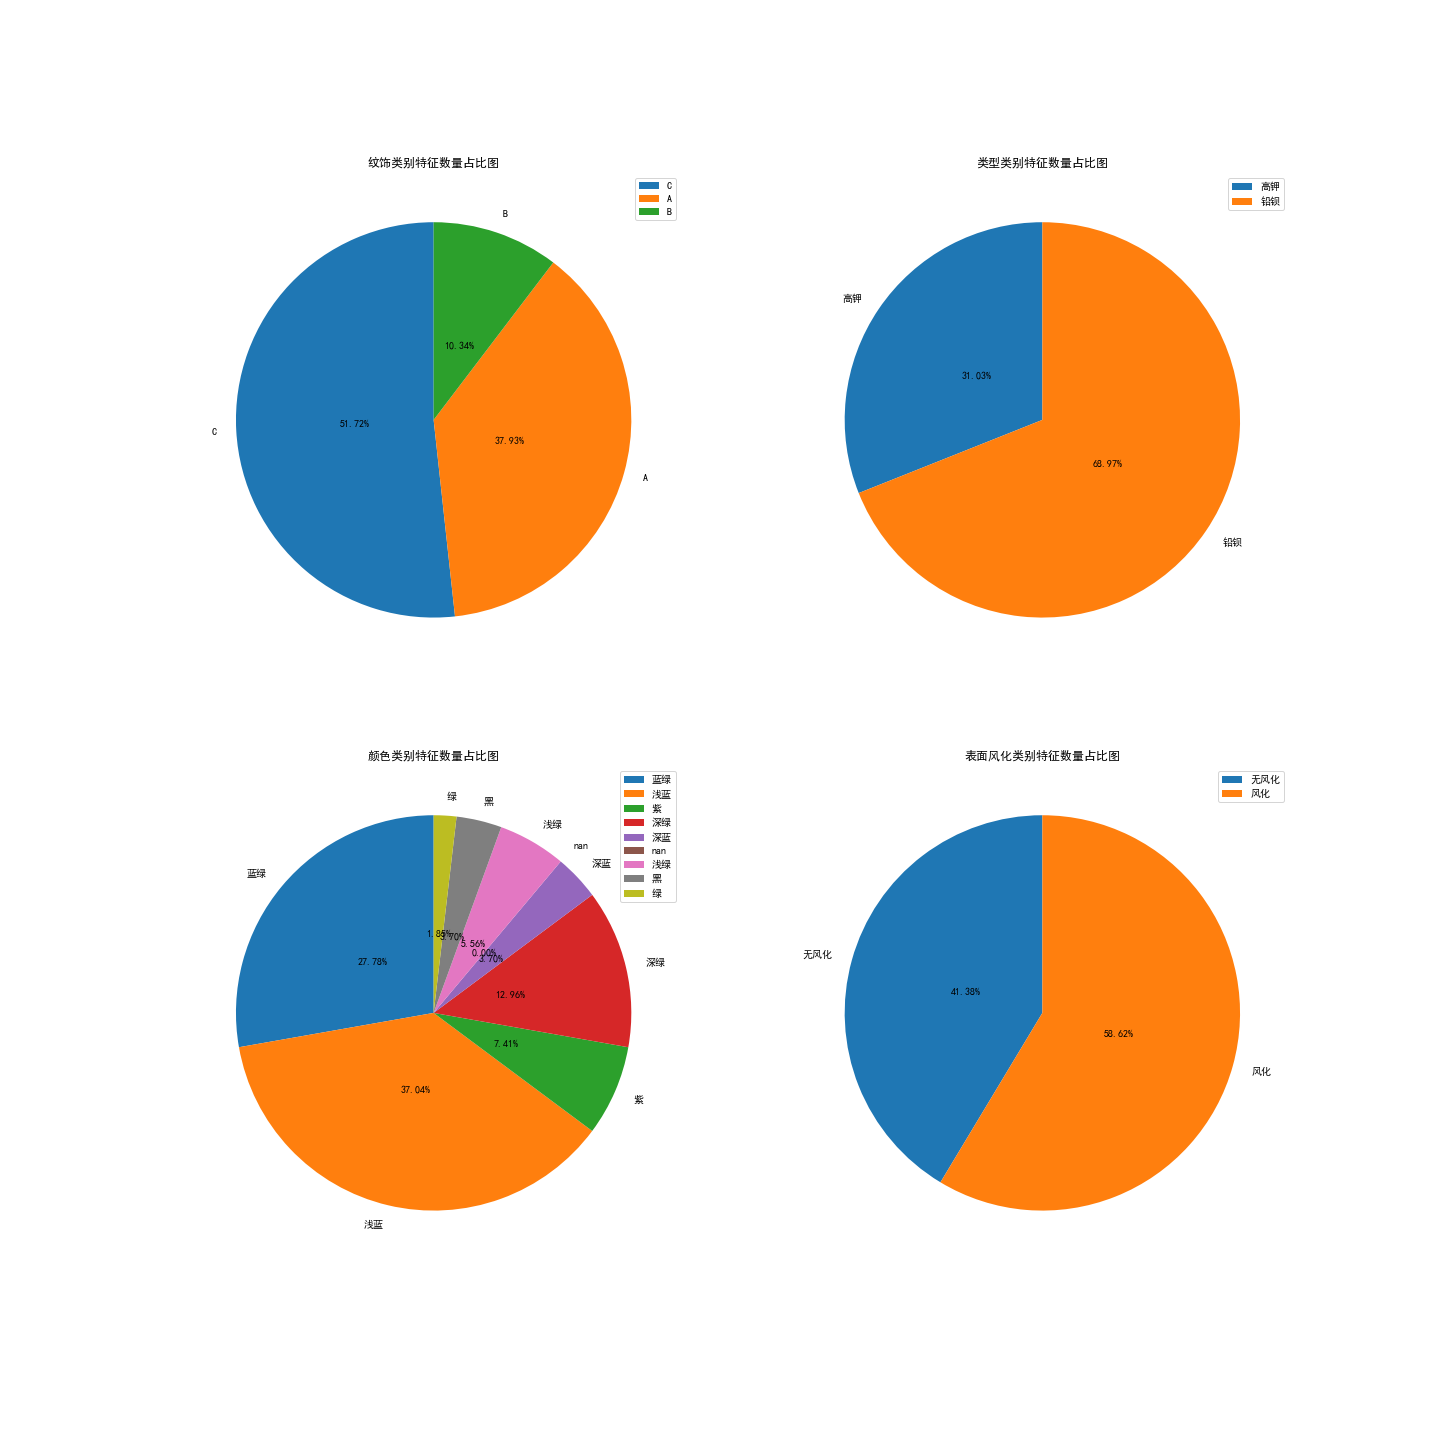
\includegraphics[width=0.8\textwidth]{ph1}
		\caption{表单1中所有类别特征的数量占比图}
		\label{fig:ph1}
	\end{figure}
	
	由图一发现,表单一中的数据中发现,古代玻璃文物制品的纹饰、类型、表面风化程度的类别特征值比较常规,而玻璃文物制品的颜色很多种,说明我国古代文物玻璃饰品的类型、纹饰分别主要由两种到三种的形式存在,玻璃文物制品的颜色多样化说明虽然我国古代的玻璃制造技术比较固定,但是可以从颜色的多样性让玻璃饰品给人们带来更多的视觉感受,也充分体现古代玻璃饰品的审美艺术气息。玻璃的成分中二氧化硅、碱(苏打、钾)和氧化钙(石灰)的比例,添加剂,如金属氧化物和乳化剂在决定材料的耐久性方面起着作用\upcite{ref1}。
	
	有了以上的分析,认为分析表面风化与其玻璃类型、纹饰和颜色的关系是非常有必要的。所以要构建表层风化—相关特征评估模型:
	
	\begin{equation}
		B_{i} = \begin{cases}
			0, & p_{i} \leq \alpha\\
			1, & p_{i} > \alpha \\
		\end{cases}
	\end{equation}

	要计算$p_{i}$的值还需要通过,计算$\chi^{2}$值,根据$pearson$卡方统计量,这里$\chi^{2}$值的公式为:
	
	\begin{equation}
		\chi^{2}_{pearson} = N\left(\sum\nolimits_{R}^{i}  \sum\nolimits_{c}^{j} \frac{A_{ij}^{2}}{\sum\nolimits_{C}^{c=i}A_{ic} \sum\nolimits_{R}^{r=1}A_{rj}}	\right) ~ \chi^{2}((R-1)(C-1))
	\end{equation}
	
	不妨假设:
	
	\centerline{\large{$H_{0}:A_{0}$ 与 $A_{i}$无关 \quad  $H_{1}:A_{0}$ 与 $A_{i}$有关}}
	
	\centerline{\large{$A_{i}$表示三个指标(玻璃类型、纹饰、颜色)中的一个指标(i=1,2,3)}}
	
	
	这里经过SPSS的$\chi^{2}$检验分析后得出关于P值的结果(表一):
	
	\begin{table}[!htb]
		\centering
		\caption{三组变量的$\chi^{2}$检验P值结果表}
		\begin{tabular}{c|c|c|c}
			\hline
			 & 玻璃类型 & 纹饰 & 颜色\\
			\hline
			表面风化 & 0.009 & 0.084 & 0.307\\
			\hline
		\end{tabular}
	\end{table}

	通过$\chi^{2}$检验得出的P-value,在置信水平α=0.05下,由表2可以看出,在统计学上,表面风化与玻璃类型有关,与纹饰和颜色无关。但是在化学角度,表面颜色是一个重要的特征,因为某些类型的退化似乎仅限于无色玻璃物体\upcite{ref1}。那么我们还需要根据相关系数corr对它们之间的关系进行进一步的分析,画出相关系数热力图(图2): 
	
	\newpage
	\begin{figure}[!h]
		\centering
		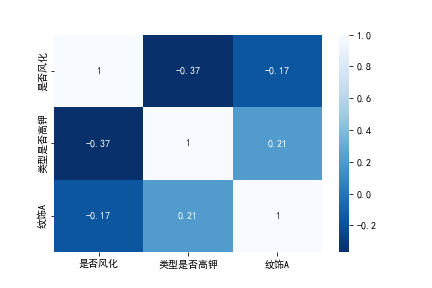
\includegraphics[width=0.8\textwidth]{ph2}
		\caption{风化与纹饰,颜色,类型四个属性的相关性热力图}
		\label{fig:ph2}
	\end{figure}
	
	结合热力图和P值结果表综合分析,得出风化与玻璃类型、颜色、纹饰呈现负相关的关系的结论,也就是说玻璃类型、颜色、纹饰是对表面风化是有影响的。也就是说明玻璃文物的表层风化与其玻璃类型、纹饰和颜色都是相关的,这里证明模型假设1是成立的。接下来找出风化的化学成分,需要将表单1和表单2的数据进行合并,合并后的数据表为表3(部分):
	
	\begin{table}[!htb]
		\centering
		\caption{表单1和表单2的合并数据(部分)}
		\begin{tabular}{cccccccccc}
			\toprule[1.5pt]
			是否风化 & 类型是否高钾&纹饰A&颜色编号&二氧化硅&氧化钠&氧化钾&……\\
			\midrule[1pt]
            0&1&0.0&0.0&71.027559 & 0.0&10.234607&……\\
            \hline
            1&0&1.0&1.0&36.319952&0.0&1.051156&……\\	
            \hline
            0&1&1.0&0.0&87.050000&0.0&5.190000&……\\	
            \hline
            0&1&1.0&0.0&62.408981&0.0&12.510113&……\\
            \hline
            0&1&1.0&0.0&68.582136&0.0&10.066625&……\\
            \hline
            …… &   ……     & ……    & ……& ……& ……& ……& …… \\
			\bottomrule[1.5pt]
		\end{tabular}
	\end{table}
	
	依据合并后的数据,画出每个化学成分与是否风化的相关性热力图,如图3所示。由于化学成分有14个之多,所以只需取5个成分(除了二氧化硅)即可,把相关系数的绝对值的大于0.21的化学成分提取出来(表4)。从表中可以看出氧化钾、 氧化钙、 氧化铁、 氧化铅、 五氧化二磷与是否风化有较大的相关关系。
	
	
	
	\begin{figure}[!h]
		\centering
		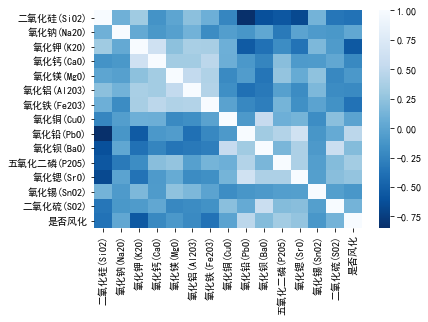
\includegraphics[width=0.8\textwidth]{ph3}
		\caption{每个化学成分与是否风化的相关性热力图}
		\label{fig:ph3}
	\end{figure}
	
	\begin{table}[!htb]
		\centering
		\caption{6个化学成分与是否风化的相关系数表}
		\begin{tabular}{ccc}
			\toprule[1.5pt]
			序号&化学成分&相关系数\\
			\midrule[1pt]
			1&二氧化硅(SiO2) &-0.373052\\
			\hline
			2&氧化钾(K2O)&-0.554855\\	
			\hline
			3&氧化钙(CaO)&-0.214721\\	
			\hline
			4&氧化铁(Fe2O3)&-0.371009\\
			\hline
			5&氧化铅(PbO)&0.480159\\
			\hline
			6&五氧化二磷(P2O5)&0.335856\\
			\bottomrule[1.5pt]
		\end{tabular}
	\end{table}

	\subsubsection{支持向量回归(SVR)风化化学成分预测模型}
	由于要根据风化点的检测数据预测其风花其风化前的化学成分含量,所以要以表面风化列的所有数据划分为两类数据,分别为未风化样品的数据和已风化样品的数据,然后根据所有未风化样品的化学成分指标数据,逐次对已风化样品数据中的单个指标建立预测算法模型,以单个未风化样品数据的所有化学成分数据作为输入,通过模型预测输出对应的风化化学成分值。
	
	\textbf{支持向量回归(SVR)预测模型的原理:}数据在间隔带内则不计算损失,当且仅当预测值f(x)与真实值y之间的差距的绝对值大于$\epsilon$才计算损失,通过最大化间隔带的宽度与最小化总损失来优化模型。SVR在线性函数两侧制造了一个“间隔带”,间距为$\epsilon$(也叫容忍偏差,是一个由人工设定的经验值),对所有落入到间隔带内的样本不计算损失,也就是只有支持向量才会对其函数模型产生影响,最后通过最小化总损失和最大化间隔来得出优化后的模型\upcite{ref3}。
	
	\begin{figure}[!h]
		\centering
		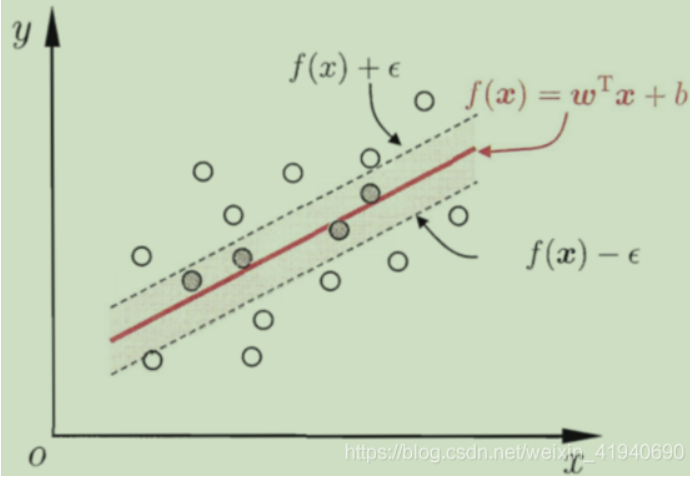
\includegraphics[width=0.8\textwidth]{ph4}
		\caption{支持向量回归模型原理图\upcite{ref3}}
		\label{fig:ph3}
	\end{figure}

	现在一个支持向量回归预测模型,由于数据是连续型和离散型混合的数据,所以我们要加入一个线性核函数,表达式为:
	
	\begin{equation}
		\kappa \left(x_{i},x_{j}\right) = x_{i}^{T} x_{j}=\phi\left(x_{i}\right)^T\phi\left(x_{j}\right)
	\end{equation}
	
	SVR模型的表达式为:
	
	\begin{equation}
		f\left(x\right) = \omega^{T}\phi\left(x\right) + b 
	\end{equation}
	
	SVR映入线性核函数之后,表达式可写为:
	 
	\begin{equation}
	    f\left(x\right) = \sum_{m}^{i=1} \alpha_{i}y_{i} \kappa \left(x,x_{i}\right)+ b 
	\end{equation}
	
	
	\begin{equation}
		\left\{  
		\begin{aligned}  
			&min \frac{1}{2}||\omega||^{2} \\  
			&s.t.|y_{i} - (\omega x_{i}+b)| \leq \epsilon,\forall i
		\end{aligned}  
		\right. 
	\end{equation}
	
	运行\textbf[附录1] 因为每一个成分都会有一个模型,所以会得到15个模型的模型系数,如图5。然后将风化后的数据放入模型预测风化前的数据即可。
	
	\begin{figure}[!h]
		\centering
		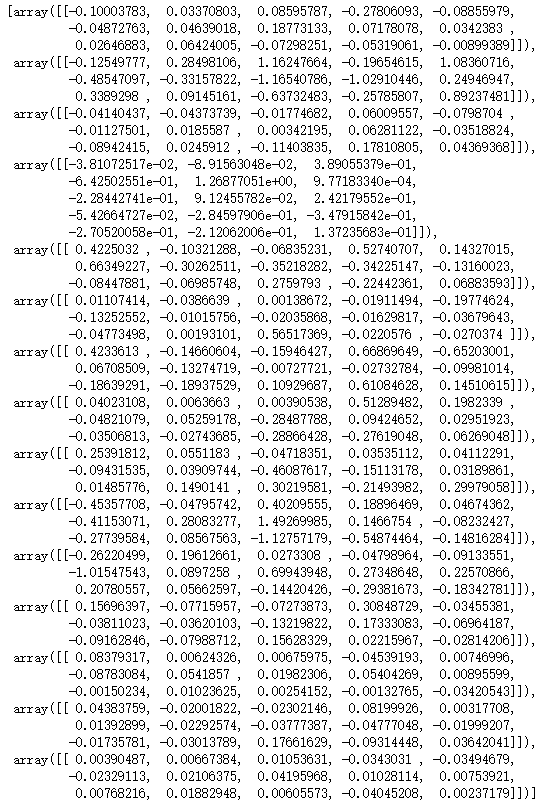
\includegraphics[width=0.8\textwidth]{ph5}
		\caption{15个模型的模型系数结果图}
		\label{fig:ph5}
	\end{figure}
	
	\subsection{问题二的求解}
	问题二要求依据数据来分析高钾玻璃、铅钡玻璃的分类规律,我们可以用K-means聚类分析算法得出高钾玻璃和铅钡玻璃的分类规律,就是根据聚类分析的结果中的两个类簇的中心的具体位置来确定高钾玻璃与铅钡玻璃是如何划分,然后根据聚类结果的准确率来判断K-means算法是否划分合理。如果划分合理,就沿用这个算法分别对高钾玻璃、铅钡玻璃进行亚类划分,然后进行聚类结果评估。流程图(图6)如下:
	
	\begin{figure}[!h]
		\centering
		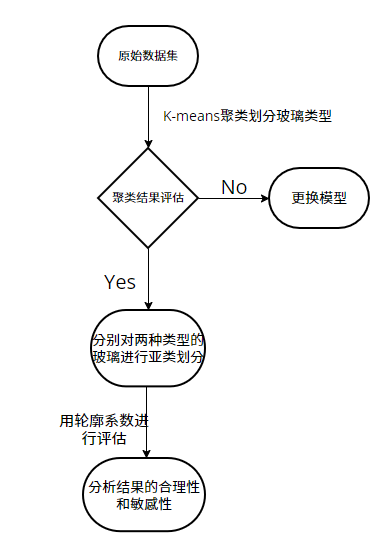
\includegraphics[width=0.8\textwidth]{ph6}
		\caption{分类过程图}
		\label{fig:ph6}
	\end{figure}
	
	\subsubsection{K-Means算法原理}
	给定样本集$D={x_{1},x_{2},...,x_{m}}$,k-means算法针对聚类所得簇划分$C = {C_{1},C_{2},...,C_{k}}$最小化平方误差
	
	\begin{equation}
		E = \sum_{k}^{i=1} ||x - \mu_{i}||_{2}^{2}
	\end{equation}
	
	其中$\mu_{i} = \frac{1}{|C_{i}|}\sum_{x \in C_{i}}x$ 是簇$C_{i}$ 的均值向量。式(7)在一定程度上
	刻画了簇内样本围绕类簇均值向量的紧密程度,E值越小则簇内样本相似度越高\upcite{ref4}。
	
	\subsubsection{K-Means算法求解}
	通过K-means算法,求解得出对于高钾玻璃和铅钡玻璃的分类结果的准确度为$73.13\%$,那么可以清楚地知道算法计算得出的类簇中心点(图7)作为聚类标准是可行的。
	
	\begin{figure}[!h]
		\centering
		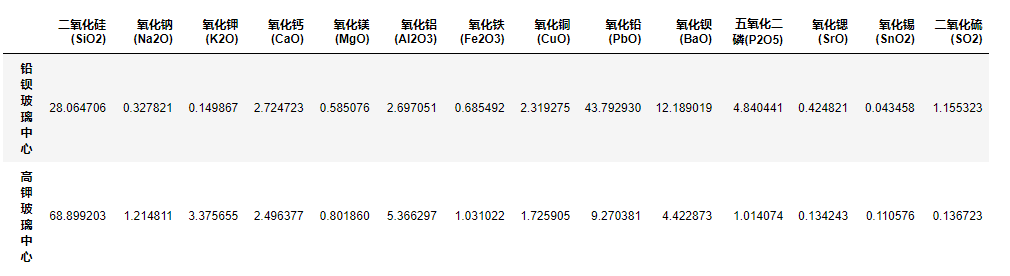
\includegraphics[width=0.8\textwidth]{ph7}
		\caption{算法求得类簇中心点位置结果图}
		\label{fig:ph7}
	\end{figure}
    
    接下来,继续使用这个算法,分别对高钾玻璃和铅钡玻璃的进行亚类划分,由于我们对于亚类的划分的类簇个数是位置的,那么我们定义k个样本作为类簇中心进行聚类,这里k的区间范围是[1,10],并画出类簇数—损失图(图8和图9)。从这两图可以观察出,铅钡玻璃亚类划分类簇个数为2时,损失数出现拐点然后摆尾;而高钾玻璃亚类划分类簇个数为3时,损失数出现拐点然后摆尾。这里有理由认为铅钡玻璃亚类划分个数应为2,高钾玻璃亚类划分个数应为3,这里给出高钾玻璃和铅钡玻璃亚类划分类簇中心的位置范围(图10和图11)。
    
    \begin{figure}[!h]
    	\centering
    	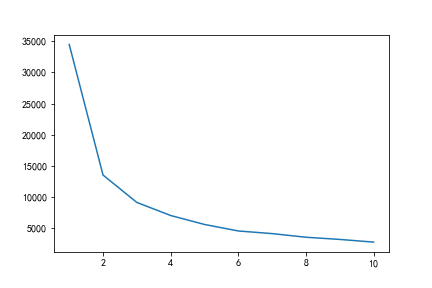
\includegraphics[width=0.8\textwidth]{ph8}
    	\caption{铅钡玻璃亚类类簇数—损失图}
    	\label{fig:ph7}
    \end{figure}

	\begin{figure}[!h]
		\centering
		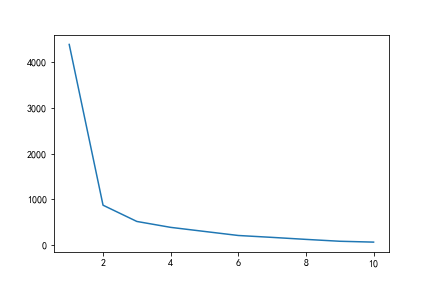
\includegraphics[width=0.8\textwidth]{ph9}
		\caption{高钾玻璃亚类类簇数—损失图}
		\label{fig:ph7}
	\end{figure}
    
    
    \clearpage
    \begin{figure}[!h]
    	\centering
    	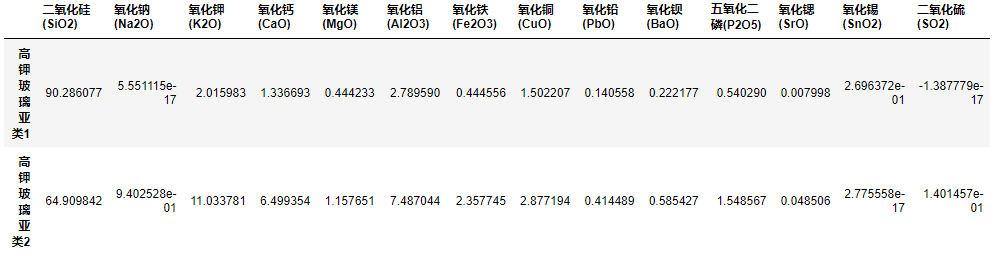
\includegraphics[width=0.8\textwidth]{ph10}
    	\caption{高钾玻璃亚类类簇中心位置范围}
    	\label{fig:ph7}
    \end{figure}

	\begin{figure}[!h]
		\centering
		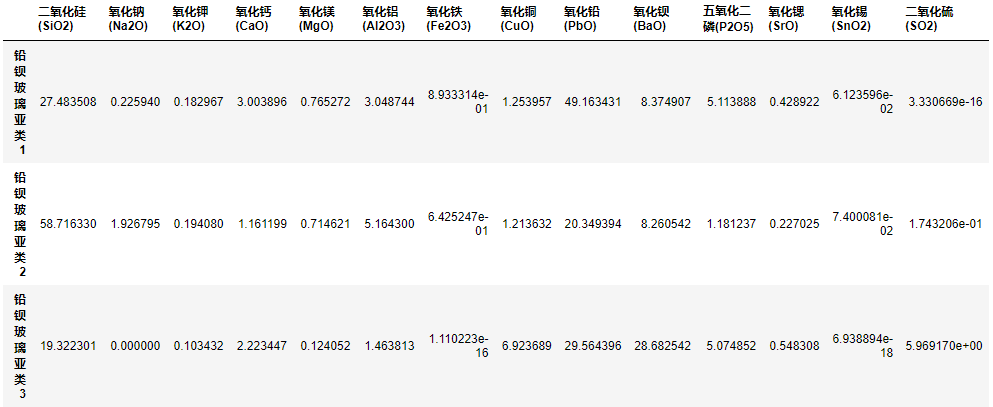
\includegraphics[width=0.8\textwidth]{ph11}
		\caption{铅钡玻璃亚类类簇中心位置范围}
		\label{fig:ph7}
	\end{figure}

	然后根据两种类型玻璃的亚类类簇中心位置作为聚类中心,进行K-means聚类,得出结果如表5:
	
	\begin{table}[!htb]
		\centering
		\caption{划分结果表(部分)}
		\begin{tabular}{cccccccccc}
			\toprule[1.5pt]
			是否风化 & 类型是否高钾&纹饰A&颜色编号&二氧化硅&氧化钠&……&亚类\\
			\midrule[1pt]
			0&1&0.0&0.0&71.027559 & 0.0&……&高钾玻璃亚类2\\
			\hline
			1&0&1.0&1.0&36.319952&0.0&……&铅钡玻璃亚类1\\	
			\hline
			0&1&1.0&0.0&87.050000&0.0&……&高钾玻璃亚类1\\	
			\hline
			0&1&1.0&0.0&62.408981&0.0&……&高钾玻璃亚类2\\
			\hline
			0&1&1.0&0.0&68.582136&0.0&……&高钾玻璃亚类2\\
			\hline
			…… &   ……     & ……    & ……& ……& ……& ……& …… \\
			\bottomrule[1.5pt]
		\end{tabular}
	\end{table}
    
    \newpage
    \subsubsection{K-Means聚类结果的合理性和敏感性}
    由于K-Means聚类属于无监督学习,而且这里我们是不知道具体的每种类型玻璃的亚类划分情况,所以这里用轮廓系数对聚类结果进行评价。\\
	\textbf{\uppercase\expandafter{\romannumeral1} 轮廓系数的定义}
	
	轮廓系数是根据内聚度和分离度这两种因素来评价聚类结果的好坏,可以用于相同的样品检测数据的基础上来评价聚类结果如何被K-means算法不同的运行方式所影响。
	\textbf{\uppercase\expandafter{\romannumeral2}轮廓系数的评估原理以及相关公式}
	
	已知轮廓系数给定大小区间为(-1,1),所以当轮廓系数越接近1时,说明聚类效果越好;反之则越差。这里给定:
	\begin{itemize}
		\item $c_{i}$:任意一个样本与其所在的类簇范围内的其他样本的平均距离(簇内不相似度)
		\item $d_{i}$:任意一个样本与其他类簇范围内的样本的平均距离(簇间相似度)\\
	\end{itemize}
	则对于任意一个样本的轮廓系数为式(8),根据簇内不相似度和簇间相似度的大小关系把式子修改为式(9),而整体的轮廓系数等于每个样本的轮廓系数之和的平均值为式(10):
	
	\begin{equation}
		s_{i} = \frac{ d_{i}-c_{i} }{max\left(c_{i},d_{i}\right)}
	\end{equation}
	
	\begin{equation}
		S_{i} =
		\begin{cases}
			1-\frac{c_{i}}{d_{i}},       & c_{i} < d_{i}\\
			0,   & c_{i} = d_{i}\\
			\frac{c_{i}}{d_{i} }- 1 ,      & c_{i} > d_{i}\\
		\end{cases}
	\end{equation}
	
	\begin{equation}
		SC = \frac{\sum_{i}^{N} S_(i)}{N}
	\end{equation}
	其中N为整体样本的个数,$S_{i}$是每个样本的轮廓系数,SC表示整体的轮廓系数。
	
	根据\textbf{[附录2]}的算法程序,计算出高钾玻璃亚类划分结果与铅钡玻璃亚类划分结果的两个整体轮廓系数(表6):
	
	\begin{table}[!htb]
		\centering
		\caption{最优亚类划分结果的轮廓系数表}
		\begin{tabular}{ccc}
			\toprule[1.5pt]
			 & 高钾玻璃亚类划分&铅钡玻璃亚类划分\\
			\midrule[1pt]
			轮廓系数&0.5674&0.5184\\
			\hline
			亚类数目&2&3\\
			\bottomrule[1.5pt]
		\end{tabular}
	\end{table}
	
	根据表6得出结论,当亚类数目是2的时候,高钾玻璃的聚类结果是最好的,当亚类数目是3的时候,高钾玻璃的聚类结果是最好的。说明了K-means聚类算法来进行亚类划分是合理的,而且敏感性良好。
	
	\subsection{问题三的求解}
	根据问题三要求,需要将表单1和表单2数据进行合并,然后以玻璃文物饰品的所有化学成分以及表面是否风化作为模型的输入变量,玻璃的类型作为模型的输出变量。用合并后的数据训练逻辑回归模型,然后用表单3的玻璃文物饰品的所有化学成分以及表面是否风化作为输入变量放入逻辑回归模型进行预测,然后输出玻璃的类型的值。然后以问题2中求出的铅钡玻璃和高钾玻璃的类簇中心位置为基准,根据表单3每个样本的数据计算与类簇中心位置距离,比较样本与两个类簇中心的距离,然后根据比较结果的来判定其所属类型,最终根据逻辑回归模型的结果与样本-类簇中心距离的匹配度,分析逻辑回归模型的分类结果的敏感性。
	
	\subsubsection{逻辑回归模型的训练与预测}
	如前文所述,我们这里用表单12的合并数据进行逻辑回归模型训练,然后进行模型预测,由于表单3数据的样本量非常小,为了防止模型过拟合,所以这里是用了基础逻辑回归模型。运行程序\textbf{[附录3]},得出预测结果整理后如下表(表7):
	
	\begin{table}[!htb]
	\centering
	\caption{逻辑回归模型预测结果}
	\begin{tabular}{ccccccccc}
		\toprule[1.5pt]
		文物编号&A1&A2&A3&A4&A5&A6&A7&A8\\
		\midrule[1pt]
		预测结果&高钾&铅钡&铅钡&铅钡&铅钡&高钾&铅钡&高钾\\
		\bottomrule[1.5pt]
	\end{tabular}
	\end{table}
	
	\subsubsection{计算表单3的样本与类簇中心的距离并判断所属类型}
	这里的类簇中心的位置如图7所示,根据距离公式(11),计算计算表单3的样本与类簇中心的距离,然后判断所属类型,运行程序[附录4],得出结果(表8):
	
	\begin{equation}
		D^{2} = \sum_{i=1}^{n}\left(x_{i}-y_{i}\right)^2
	\end{equation}
	其中,$D^{2}$为某个样本与类簇中心点的距离的平方和,$x_{i}$为样本的第i个数据,$y_{i}$为类簇中心点的第i个数据
	
	\begin{table}[!htb]
	\centering
	\caption{根据距离判断结果}
	\begin{tabular}{ccccccccc}
		\toprule[1.5pt]
		文物编号&A1&A2&A3&A4&A5&A6&A7&A8\\
		\midrule[1pt]
		判断结果&高钾&铅钡&铅钡&铅钡&高钾&高钾&高钾&高钾\\
		\bottomrule[1.5pt]
	\end{tabular}
	\end{table}
	
	\subsubsection{分析逻辑回归模型预测结果的敏感性}
	将表7和表8的数据进行合并,根据匹配结果分析分类结果的敏感性,然后记1为匹配成功,0为匹配失败,如表9所示:
	
	\begin{table}[!htb]
		\centering
		\caption{匹配结果}
		\begin{tabular}{ccccccccc}
			\toprule[1.5pt]
			文物编号&A1&A2&A3&A4&A5&A6&A7&A8\\
			\midrule[1pt]
			预测结果&高钾&铅钡&铅钡&铅钡&铅钡&高钾&高钾&铅钡\\
			\hline
			判断结果&高钾&铅钡&铅钡&铅钡&高钾&高钾&高钾&高钾\\
			\hline
			匹配结果&1&1&1&1&0&1&1&0\\
			\bottomrule[1.5pt]
		\end{tabular}
	\end{table}
	
	从表9的匹配结果看出,匹配成功率为$75\%$,等价于验证准确度为$75\%$,结合判断结果和预测结果,可以认为逻辑回归模型的分类预测结果的敏感性是良好的。
	
	\subsection{问题四的求解}
	题目四要求分析不同类型玻璃的化学成分之间的关联关系,不用考虑是否风化,则这里使用表单12合并后数据中的类型和所有化学成分的数据做关联分析。所以这里我采用了方差分析算法来分析不同类别玻璃、化学成分之间的关系。运行程序\textbf{[附录4]},得到以下结果,如表10所示:
	
	\begin{table}[!htb]
		\centering
		\caption{方差分析结果}
		\begin{tabular}{cccccc}
			\toprule[1.5pt]
			&df	&sum\_sq	&mean\_sq&F&PR(>F)\\
			\midrule[1pt]
			C(类型是否高钾)&14.0&172415.149547&12315.367825&162.425542&8.414966e-245\\
			\hline
			Residual&990.0&75063.404636&75.821621&NaN&NaN\\
			\bottomrule[1.5pt]
		\end{tabular}
	\end{table}
	我们可以看到不同玻璃类型,对于化学成分的影响还是十分显著的,p值显然小于0.05
	
	然后进行差异性分析,运行程序\textbf{[附录4]},得到相关结果,展示部分结果(图12):
	\begin{figure}[!h]
		\centering
		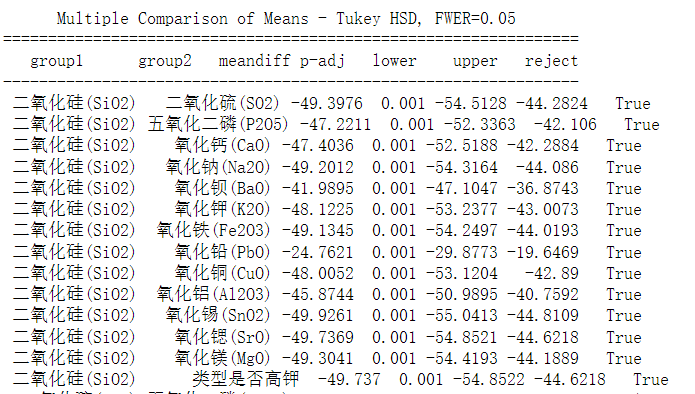
\includegraphics[width=0.8\textwidth]{ph12}
		\caption{不同类别之间的化学成分关联关系的差异性(部分)}
		\label{fig:ph12}
	\end{figure}
	
	从分析相关性和观察运行结果图而知,不同玻璃类型的化学成分相互影响,尤其是二氧化硫对二氧化硅的影响最大,二氧化硫与水结合生成亚硫酸会腐蚀破坏玻璃制品的表层结构,从而使其风化的程度更严重。通过差异性分析,我们还知道不同玻璃类型的化学成分是有差异的,助熔剂、添加剂的成分不同促使其化学成分的关联关系,所以玻璃的制造工艺决定玻璃制品的化学成分含量具备差异性。
	
	\section{模型分析}
	\subsection{模型的优点}
	\begin{itemize}
		\item[1.] 从数据挖掘的方向入手,运用卡方检验进行统计分析,可以从数据中找到隐含规律;
		\item[2.] 在数据的数量极其少情况下,结合逻辑回归模型与k-means算法,能够较好判别文物的类型;
		\item[3.] 支持向量回归(SVR)预测模型有效地预测出玻璃文物风化前的化学成分数据;
		\item[4.] 在未知亚类的类别数目的情况下,使用无监督学习算法K-means,以及轮廓系数对于聚类结果的评估,能够较好地解释亚类的划分结果。
	\end{itemize}
	
	\subsection{模型的缺点}
	\begin{itemize}
		\item[1.] 仅适用于数据量较小的数据集,数据量较大的话模型可能会失去作用,模型的准确度也会有所下降。
		\item[2.] 模型并未添加风险因素,古代文物玻璃制品中不同的埋藏条件决定着不同类型的风化作用,也会影响化学成分的变化。
	\end{itemize}
	
	
	
	
	
	%参考文献i
	\clearpage
	\section{参考文献与引用}
	\begin{thebibliography}{8}%宽度8
		\bibitem{ref1}
		Gueli AM, Pasquale S, Tanasi D, et al. Weathering and deterioration of archeological glasses from late Roman Sicily. Int J Appl Glass Sci. 2019;00:1–11. 
		\bibitem{ref2}
		姜启源, 谢金星, 叶俊. 数学模型 [M]. 北京: 高等教育出版社, 2003.
		\bibitem{ref3}
		支持向量回归(SVR)的详细介绍以及推导算法\url{https://blog.csdn.net/weixin_41940690/article/details/106639347}
		\bibitem{ref4}
		机器学习/周志华著•-北京:清华大学出版社,2016
		\bibitem{ref5}
		Peter J. Rousseeuw,
		Silhouettes: A graphical aid to the interpretation and validation of cluster analysis,
		Journal of Computational and Applied Mathematics,
		Volume 20,
		1987
	\end{thebibliography}

	\newpage
	%附录
	\begin{appendices}
	
	\section{附录}
	\subsection{支撑材料清单}
	\begin{itemize}
		\item 玻璃文物的表面风化与纹饰的交叉表和卡方检验.docx
		\item ph1.png
		\item ph2.png
		\item ph3.png
		\item ph4.png
		\item ph5.png
		\item ph6.png
		\item ph7.png
	    \item ph8.png
        \item ph9.png
        \item ph10.png
        \item ph11.png
        \item ph12.png
        \item ph12.png
		\item k-means.py
		\item SVR风化化学成分预测模型.py
		\item 方差分析.py
		\item 逻辑回归模型.py
		\item 表单12合并汇总.xlsx
	\end{itemize}
	
	
	\subsection{附录1:SVR风化化学成分预测模型.py}
	\begin{lstlisting}
		#导入相关库
		import pandas as pd
		import numpy as np
		from sklearn import svm
		
		#导入合并后的数据集
		data = pd.read_excel(r"表单12数据合并汇总.xlsx")
		
		#划分两类数据集,风化文物饰品的数据和未风化文物饰品数据
		fenghua = data[data['表面风化']==1]
		weifenghua = data[data['表面风化']==0]
		cols = ['类型是否高钾']+list(df.columns[6:])
		fenghua = fenghua[cols]
		weifenghua = weifenghua[cols]
		#支持向量回归SVR模型
		svr = svm.SVR(kernel='linear')
		
		#模型训练
		cf = [0 for i in range(len(cols))]
		for i in range(len(cols)):
		for j in range(5):
		index = list(fenghua.index)
		np.random.shuffle(index)
		svr.fit(fenghua.loc[index[:25]].values, weifenghua.values[:, i])
		cf[i] += svr.coef_/5
		for i in range(15):
		print(fenghua.columns[i], '的模型系数',cf[i])
	\end{lstlisting}
	
	\subsection{附录2:k-means.py}
	\begin{lstlisting}
		#导入相关库
		import pandas as pd
		import numpy as np
		from sklearn.cluster import k_means
		
		#导入合并后的数据集
		data = pd.read_excel(r"表单12数据合并汇总.xlsx")
		
		cols = df.columns[6:]
		KMS = k_means(df[cols], 2)
		KMS
		
		accuracy = (KMS[1]==df['类型是否高钾']).sum()/len(df)*100
		accuracy
		
		#求出高钾玻璃和铅钡玻璃类型划分中心
		category_1 = pd.DataFrame(KMS[0],columns = cols, index = ['铅钡玻璃中心','高钾玻璃中心'])
		category_1
		
		#划分高钾玻璃亚类
		gaojia = df[df['类型是否高钾']==1]
		category_2 = k_means(gaojia[gaojia.columns[6:]], 2)
		category_2 = pd.DataFrame(data=category_2[0], columns=[gaojia.columns[6:]], index=['高钾玻璃亚类1','高钾玻璃亚类2'])
		category_2
		
		#划分铅钡玻璃亚类
		qianbei = df[df['类型是否高钾']==0]
		category_3 = k_means(qianbei[qianbei.columns[6:]], 3)
		category_3 = pd.DataFrame(data=category_3[0], columns=[qianbei.columns[6:]], index=['铅钡玻璃亚类1','铅钡玻璃亚类2','铅钡玻璃亚类3'])
		category_3
		
		#计算整体轮廓系数
		from sklearn.metrics import silhouette_score
		Silhouette_Coefficient1 = silhouette_score(gaojia[gaojia.columns[6:]], category_2[1])
		Silhouette_Coefficient1
		
		Silhouette_Coefficient2 = silhouette_score(qianbei[qianbei.columns[6:]], category_3[1])
		Silhouette_Coefficient2
	\end{lstlisting}

	\subsection{附录3:逻辑回归模型.py}
	\begin{lstlisting}
		import numpy as np
		import pandas as pd
		from sklearn.linear_model import LogisticRegression 
		
		data = pd.read_excel('表单12数据合并汇总.xlsx', index_col=0)
		#附件表单3的数据处理
		data1 = pd.read_excel('附件.xlsx', index_col=2)
		data1=data1.fillna(0)
		cols1 = data1.columns[2:]
		data1['成分比例累加和']=np.sum(data1[cols1], axis=1)
		
		cols = data.columns[6:]
		x_tr = data[['是否风化']+list(cols)].values
		y_tr = data['类型是否高钾'].values
		
		pre = data1[data1.columns[1:-1]].values
		LogisticRegression.fit(x_tr, y_tr)
		pre_y = LogisticRegression.predict(pre)
		pre_y
	\end{lstlisting}	

	\subsection{附录4:方差分析.py}
	\begin{lstlisting}
		import pandas as pd
		import numpy as np
		
		data = pd.read_excel(r"表单12数据合并汇总.xlsx", index_col=0)
		col = ['类型是否高钾','二氧化硅(SiO2)',
		'氧化钠(Na2O)', '氧化钾(K2O)', '氧化钙(CaO)', '氧化镁(MgO)', '氧化铝(Al2O3)',
		'氧化铁(Fe2O3)', '氧化铜(CuO)', '氧化铅(PbO)', '氧化钡(BaO)', '五氧化二磷(P2O5)',
		'氧化锶(SrO)', '氧化锡(SnO2)', '二氧化硫(SO2)']
		data1 = data[col]
		
		# 方差分析
		from statsmodels.formula.api import ols
		from statsmodels.stats.anova import anova_lm
		from statsmodels.stats.multicomp import pairwise_tukeyhsd
		
		data_melt = data1.melt()
		data_melt.columns = ['类型是否高钾', '化学成分']
		model = ols('化学成分 ~C(类型是否高钾)', data = data_melt).fit()
		anova_table = anova_lm(model, type = 2)
		pd.DataFrame(anova_table)
		
		# 进行事后比较分析
		print(pairwise_tukeyhsd(data_melt['化学成分'], data_melt['类型是否高钾']))
	\end{lstlisting}	
	\end{appendices}
\end{document}